% Discuter les résultats, sources d'incertitudes, ...

Tout au long des expérience, nos résultats sont pertinents et intéressants. Notons avant d'entrer dans une analyse plus fine une bonne précision dans la mesure, malgré quelques sources d'incertitudes. La première est le bruit du teslamètre mentionné au début de la section précédente. De plus, nous avons considérer les mesures propres au solénoïde comme acquise et ne les avons pas vérifier, ni pris garde à leur précision. Finalement, le dispositif n'est pas parfait non plus, la bobine qui chauffe par exemple peut modifier certaines propriétés, et la présence de beaucoup de matériel produisant un champ électromagnétique dans le laboratoire induit un peu d'erreur en plus.\\ \\
Par la première expérience, nous constatons que le modèle issue de l'analyse différentiel du problème est très proche des mesures, quoiqu'un peu au-dessus, qui peut s'expliquer par un petit décalage du teslamètre vis à vis du centre du solénoïde entre autres hypothèses. Celle-ci découle des résultats de la seconde expérience montrant la diminution du champs magnétique avec le décalage.\\ \\
De plus, la version simplifiée fonctionne bien quand on s'approche du solénoïde parfait, mais dès que l'on est plus proche d'une petite bobine, cela ne donne plus de résultat pertinent. Dans le cas de notre expérience, on peut poser une limite autour de 50 spires, au-dessus de laquelle l'erreur est inférieur à $5 \ [\%]$ et devient une excellente approximations. Nous voyons la différence entre les deux versions, ainsi que les variables pour lequel elles se valent sur le graphe comparant leurs erreurs relatives.\\
En étudiant la différence entre la droite représentant le calcul du champs par l'approximation sur les points considérant les mesures fournies par le fabriquant, et ceux considérant le nombre de spires proportionnel à la distance, on peut soit supposer une incertitude dans les données, ou une fabrication du solénoïde qui n'est pas parfaitement régulière.\\ \\
Sur la seconde expérience, nous pouvons supposer un champs magnétique ambiant ou des spécifications du solénoïde menant à des points de mesures plus faibles que la théorie, ainsi qu'à une diminution plus tardive de celui-ci. Ce deuxième effet peut aussi s'expliquer par un décentrage du teslamètre dans le solénoïde.\\ \\
Entre les deux expérience, nous observons que le modèle analytique du problème permet de décrire très fidèlement la réalité avec une erreur relative inférieure à $3 \ [\%]$ pour les valeurs assez grandes, et sinon on observe malgré tout une erreur absolue de l'ordre de grandeur du bruit apparaissant sur le teslamètre et cela apparaît donc comme une grande proportion mais ce sont plutôt des mesures pour lequel le matériel n'est pas tout à fait adapter.\\ \\
Mais on peut se dire que le résultat n'est pas exacte. En effet, on a considéré pour produire le résultat analytique en considérant le solénoïde comme une somme de cercle infinitésimaux, or c'est une courbe plus complexe et chaque enroulement crée une légère déformation du champs, visible sur la figure ci-dessous, que l'on ne prend pas en compte par ce calcul. Nous observons malgré tout que pour le centre de la bobine, c'est tellement proche de la réalité que l'on peut considérer cela comme exacte.\\

\begin{invsummary}
La simulation du champs magnétique d'un solénoïde présentée ci-dessous a été réalisée numériquement via la loi de Biot-Savart de laquelle on tire la relation suivante :
$$\vec{B}(\vec{r}) =  \frac{\mu_0 I}{4 \pi} \int_C \frac{d\vec{l} \times (\vec{r}-\vec{l})}{|\vec{r}-\vec{l}|^3} $$
avec $C$ la courbe que l'on considère, $\vec{l}$ la direction sur la courbe et $\vec{r}$ le vecteur position.\\ \\
Sachant qu'un solénoïde peut être décrit par la courbe paramétrique suivante :
$$ \vec{l}(t) = \begin{pmatrix}
R \cdot \sin t \\
R \cdot \cos t \\
\alpha t
\end{pmatrix} $$
avec $R$ le rayon et $\alpha$ un scalaire réglant l'espace entre deux révolution.\\ \\
On peut donc faire $n$ rotations en prenant $t \in \left[0 ; 2 n \pi \right]$, puis obtenir le champs via une intégration numérique assez aisée sur ordinateur\footnotemark :
$$\vec{B}(\vec{r}) = \int_0^{2 n \pi} \frac{d\vec{l}/dt \times (\vec{r} - \vec{l})}{|\vec{r}-\vec{l}|^3} dt$$
\end{invsummary} \footnotetext{Code inspiré d'un \href{https://github.com/lukepolson/youtube_channel/blob/main/Python\%20Metaphysics\%20Series/vid12.ipynb}{notebook} mis en ligne par \href{https://www.youtube.com/@MrPSolver}{Mr. P Solver}, vidéo : \href{https://www.youtube.com/watch?v=srk2YZKMn-E}{https://www.youtube.com/watch?v=srk2YZKMn-E}}
\begin{figure}[H]
\centering
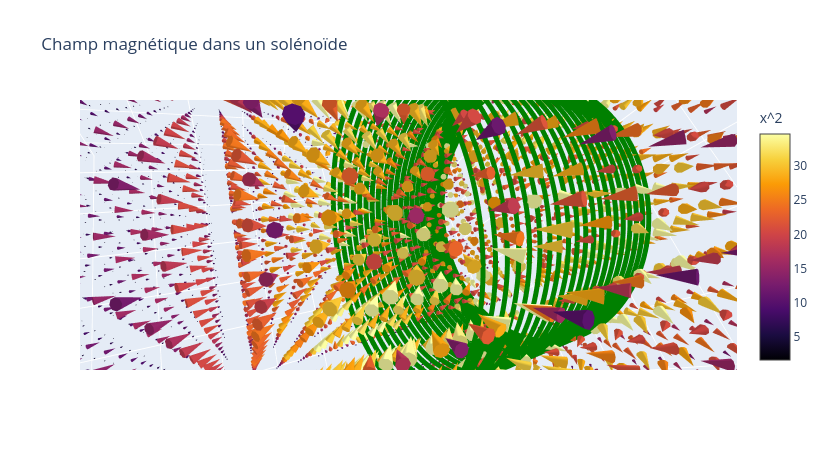
\includegraphics[width=.8\textwidth]{magnetic_field.png}

\caption{Simulation du champs magnétique produit par un solénoïde}
\end{figure}